
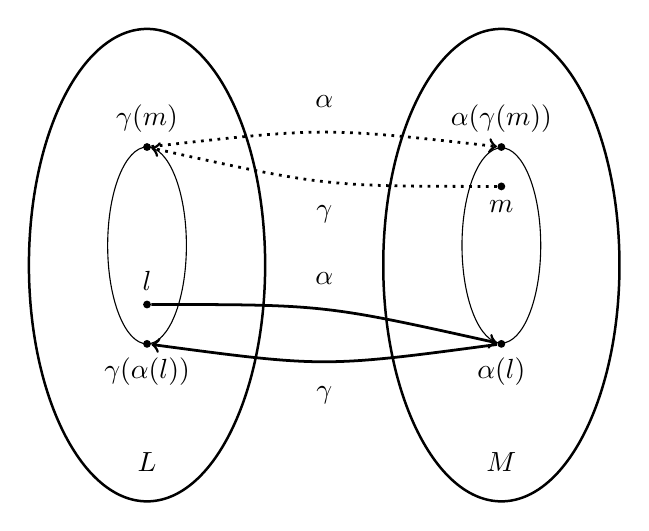
\begin{tikzpicture}

\draw[line width=0.9pt] (1.5,3) ellipse (1.5 and 3);
\draw[line width=0.9pt] (6,3) ellipse (1.5 and 3);


\draw (1.5,4.5) node[circle,fill,inner sep=1pt,label=above:$\gamma(m)$](gammam){};
\draw (1.5,2.5) node[circle,fill,inner sep=1pt,label=above:$l$](l){};
\node(L) at (1.5,0.5) {$L$};
\draw (1.5, 3.25) ellipse (0.5 and 1.25);
\draw (l) node[yshift=-0.5cm, circle,fill,inner sep=1pt,label=below:$\gamma(\alpha(l))$](gammaalphal){};

\draw (6,4) node[circle,fill,inner sep=1pt,label=below:$m$](m){};
\draw (6,2) node[circle,fill,inner sep=1pt,label=below:$\alpha(l)$](alphal){};
\node(L) at (6,0.5) {$M$};
\draw (6, 3.25) ellipse (0.5 and 1.24);
\draw (m) node[yshift=0.5cm, circle,fill,inner sep=1pt,label=above:$\alpha(\gamma(m))$](alphagammam){};

\draw (3.75,2.5) node[label=above:$\alpha$](alpha) {};
\draw[->, line width=1pt] (l) .. controls  (alpha) .. (alphal);

\draw (3.75,1.7) node[label=below:$\gamma$] (gamma) {};
\draw[->, line width=1pt] (alphal) .. controls  (gamma) .. (gammaalphal);


\draw (3.75,4.75) node[label=above:$\alpha$](alpha0) {};
\draw (3.75,4) node[label=below:$\gamma$](gamma0) {};

\draw[->, dotted, line width=1pt] (m) .. controls (gamma0) .. (gammam);
\draw[->, dotted, line width=1pt] (gammam) .. controls (alpha0) .. (alphagammam);


\end{tikzpicture}

